% !TeX program = lualatex
% ============================================================================
% Monografia — TCC UPE-POLI 2026.1 (modelo abnTeX2 da ECOMP-POLI)
% Template: preencha seus dados em pretextuais/capa.tex
% ============================================================================
\documentclass[
    section=TITLE,      % títulos de seções em maiúsculas
    12pt,
    oneside,
    a4paper,
    english,            % idioma adicional (resumo em inglês)
    brazil              % idioma principal
]{monografia-abntex2}

% --- Pacotes básicos ---
\usepackage{fontspec}
\IfFileExists{fonts/Arial/Arial.ttf}{%
    \setmainfont{Arial}[
        Path=./fonts/Arial/,
        UprightFont=Arial.ttf,
        BoldFont=Arial_Bold.ttf,
        ItalicFont=Arial_Italic.ttf,
        BoldItalicFont=Arial_Bold_Italic.ttf
    ]%
    \setsansfont{Arial}[
        Path=./fonts/Arial/,
        UprightFont=Arial.ttf,
        BoldFont=Arial_Bold.ttf,
        ItalicFont=Arial_Italic.ttf,
        BoldItalicFont=Arial_Bold_Italic.ttf
    ]%
}{%
    \setmainfont{Arial}%
    \setsansfont{Arial}%
}
\usepackage{lastpage}
\usepackage{indentfirst}
\usepackage{color}
\usepackage{graphicx}
\usepackage{float}
\usepackage{amsmath,amssymb}
\usepackage{booktabs}
\usepackage{tabularx}
\usepackage{caption}
\usepackage{subcaption}
\usepackage{enumitem}
\usepackage{algorithm}        % ambiente flutuante para algoritmos
\usepackage{algpseudocode}    % pseudocódigo (algorithmicx)
\usepackage{tikz}             % fluxograma da metodologia
\usetikzlibrary{positioning, arrows.meta}

% --- Algoritmos em português ---
\floatname{algorithm}{Algoritmo}
\renewcommand{\listalgorithmname}{Lista de algoritmos}
\algrenewcommand\algorithmicrequire{\textbf{Entrada:}}
\algrenewcommand\algorithmicensure{\textbf{Saída:}}
\algrenewcommand\algorithmicfor{\textbf{para}}
\algrenewcommand\algorithmicforall{\textbf{para todo}}
\algrenewcommand\algorithmicdo{\textbf{faça}}
\algrenewcommand\algorithmicwhile{\textbf{enquanto}}
\algrenewcommand\algorithmicend{\textbf{fim}}
\algrenewcommand\algorithmicif{\textbf{se}}
\algrenewcommand\algorithmicthen{\textbf{então}}
\algrenewcommand\algorithmicelse{\textbf{senão}}
\algrenewcommand\algorithmicreturn{\textbf{retorne}}

% --- Citações ABNT (autor-data, backend bibtex) ---
\usepackage[alf,abnt-repeated-title-omit=yes,abnt-emphasize=bf,abnt-etal-list=0]{abntex2cite}
\usepackage{pdfpages}

% Sumário: entrada REFERÊNCIAS recuada à coluna dos títulos de capítulo
% (deck ECOMP "Formatação final", slides 27-30: não alinhar Referências à margem)
\renewcommand{\bibsection}{%
  \chapter*{\bibname}
  \bibmark
  \ifnobibintoc\else
  \phantomsection
  \addcontentsline{toc}{chapter}{\texorpdfstring{\protect\numberline{}\MakeTextUppercase{Referências}}{Referências}}
  \fi
  \prebibhook
}
\citebrackets()

% --- Diretórios de imagens ---
\graphicspath{{imagens/}{figuras/}}

% --- Fonte de figuras/tabelas (ABNT) ---
\newcommand{\source}[1]{\par\vspace{2pt}{\footnotesize\textbf{Fonte:} #1}\par}

% --- Dados do trabalho (capa e folha de rosto) ---
% ---
% Informações de dados para CAPA e FOLHA DE ROSTO
% ---
\titulo{Título do Trabalho}
\autor{André Gustavo Vasconcelos Escorel Ribeiro}
\local{Recife}
\data{2026}
\orientador{Prof. Dr. Ricardo Ataíde}
\instituicao{
  Universidade de Pernambuco \\
  \vspace{1mm}
  Escola Politécnica de Pernambuco \\
  \vspace{2mm}
  Graduação em Engenharia de Computação
}
\tipotrabalho{
  Trabalho de Conclusão de Curso \\
  \SingleSpacing
  Engenharia de Computação
}
% O preâmbulo deve conter o tipo do trabalho, o objetivo,
% o nome da instituição e a área de concentração.
\preambulo{Monografia apresentada como requisito parcial para obtenção do diploma de Bacharel em Engenharia de Computação pela Escola Politécnica de Pernambuco -- Universidade de Pernambuco.}
% ---


% --- Informações do PDF ---
\makeatletter
\hypersetup{
    pdftitle={\@title},
    pdfauthor={\@author},
    pdfsubject={\imprimirpreambulo},
    pdfcreator={LaTeX with abnTeX2},
    colorlinks=true,
    linkcolor=black,
    citecolor=black,
    urlcolor=blue,
    bookmarksdepth=4
}
\makeatother

% --- Espaçamentos ---
\setlength{\parindent}{1.25cm}
\setlength{\parskip}{0pt}

% ============================================================================
\begin{document}
\selectlanguage{brazil}
\frenchspacing

% ----------------------------------------------------------
% ELEMENTOS PRÉ-TEXTUAIS
% ----------------------------------------------------------
\imprimircapa
\imprimirfolhaderosto

% Elementos obtidos pós-defesa / depósito:
% Ficha catalográfica (verso da folha de rosto).
% Ao inserir, manter o \addtocounter: capa e ficha NÃO contam na numeração (regra ECOMP).
%\includepdf{pretextuais/ficha_catalografica.pdf}\addtocounter{page}{-1}
%\includepdf{pretextuais/folha_aprovacao.pdf}        % Avaliação Final assinada pela banca
%\includepdf{pretextuais/termo_autorizacao.pdf}      % autorização de divulgação assinada

% Resumo e Abstract
% resumo em português (150-500 palavras, parágrafo único, 3-5 palavras-chave)
% O texto abaixo está comentado; remova o "%" de cada linha para publicar.
\setlength{\absparsep}{18pt}
\begin{resumo}
% Este trabalho desenvolveu e avaliou um soft-sensor embarcado para estimar a
% potência ativa CA de inversores fotovoltaicos a partir de variáveis
% meteorológicas, cobrindo falhas de telemetria. Os dados vieram da Rede
% Solarimétrica de Pernambuco, com três inversores de 2~kW. O conjunto foi
% preparado em quatro granularidades (5~min, 10~min, 1~h e 1~d), com
% separação temporal entre treino, calibração e teste. Dois modelos foram
% comparados: Random Forest e perceptron de múltiplas camadas. Os modelos
% foram treinados, avaliados no teste de 2025 e embarcados em um ESP32-S3,
% com bibliotecas geradas por emlearn e TensorFlow Lite. No teste, o MLP
% apresentou MAE entre $0{,}160$ e $0{,}037$~kW e R$^2$ entre $0{,}808$ e
% $0{,}981$; o Random Forest ficou próximo, com MAE entre $0{,}164$ e
% $0{,}040$~kW e R$^2$ entre $0{,}805$ e $0{,}972$, e menor custo de
% memória. A análise cruzada mostrou que um modelo treinado em 1~h manteve
% R$^2$ de $0{,}784$ (MLP) e $0{,}777$ (RF) quando avaliado em 5~min. No
% ensaio na placa, o Random Forest de 1~h reproduziu o resultado
% \textit{offline}, com MAE de $0{,}066$~kW fora dos \textit{gaps} e
% $0{,}065$~kW dentro deles, contra $0{,}312$~kW da interpolação linear e
% $0{,}376$~kW da persistência. O resultado indica que o soft-sensor cobre a
% lacuna de telemetria com erro próximo do normal e muito abaixo das
% baselines, e que o caminho embarcado não degrada a inferência.
%
% \textbf{Palavras-chave:} aprendizado de máquina; sistemas fotovoltaicos;
% soft-sensor; ESP32-S3; dados faltantes.
\end{resumo}

% resumo em inglês
\begin{resumo}[Abstract]
\begin{otherlanguage*}{english}
% This work developed and evaluated an embedded soft sensor that estimates
% the AC active power of photovoltaic inverters from meteorological
% variables, covering telemetry failures. The data came from the
% Pernambuco Solarimetric Network, with three 2~kW inverters. The dataset
% was prepared at four granularities (5~min, 10~min, 1~h and 1~d), with a
% temporal split between training, calibration and test. Two models were
% compared: Random Forest and a multilayer perceptron. The models were
% trained, evaluated on the 2025 test set and deployed on an ESP32-S3, with
% libraries generated by emlearn and TensorFlow Lite. On the test set, the MLP
% reached an MAE between $0.160$ and $0.037$~kW and an R$^2$ between
% $0.808$ and $0.981$; the Random Forest was close, with an MAE between
% $0.164$ and $0.040$~kW and an R$^2$ between $0.805$ and $0.972$, and a
% lower embedded cost. The cross-granularity analysis showed that a model
% trained at 1~h kept an R$^2$ of $0.784$ (MLP) and $0.777$ (RF) when
% evaluated at 5~min. In the board test, the 1~h Random Forest reproduced
% the offline result, with an MAE of $0.066$~kW outside the gaps and
% $0.065$~kW inside them, against $0.312$~kW for linear interpolation and
% $0.376$~kW for persistence. The result indicates that the soft sensor
% covers the telemetry gap with an error close to the normal one and well
% below the baselines, and that the embedded path does not degrade the
% inference.
%
% \textbf{Keywords:} machine learning; photovoltaic systems; soft sensor;
% ESP32-S3; missing data.
\end{otherlanguage*}
\end{resumo}


% Listas
\pdfbookmark[0]{\listfigurename}{lof}
\listoffigures*
\cleardoublepage

\pdfbookmark[0]{\listtablename}{lot}
\listoftables*
\cleardoublepage

% Sumário
\pdfbookmark[0]{\contentsname}{toc}
\tableofcontents*
\cleardoublepage

% ----------------------------------------------------------
% ELEMENTOS TEXTUAIS
% ----------------------------------------------------------
\textual

% ============================================================================
% RASCUNHO COMENTADO: Introdução
% Para publicar, remova o "%" do início de cada linha.
% ============================================================================
%
\chapter{Introdução}
\label{cap:introducao}
%
% A geração fotovoltaica conectada à rede depende de medições contínuas para
% acompanhar a produção, detectar falhas e gerir a usina. Em uma usina
% monitorada, cada inversor reporta a potência ativa entregue à rede, e essa
% série alimenta os indicadores de desempenho. Quando a telemetria falha, o
% registro desaparece, e a lacuna compromete a contabilidade da geração, o
% cálculo de indicadores e a identificação de anomalias.
%
% O problema aparece nos dados da Rede Solarimétrica de Pernambuco
% (RedeSolarPE), mantida pelo Instituto Federal de Pernambuco (IFPE),
% \textit{campus} Pesqueira, que consolida registros operacionais de usinas
% fotovoltaicas conectadas à rede no estado
% \cite{pedrosafilho2022,pedrosafilho2025}. Nos três inversores de 2~kW
% analisados neste trabalho, E1, E2 e E3, a fração de períodos diurnos sem
% registro fica em torno de 13,5\%, e a maior lacuna contínua chega a 12~h.
%
% A proposta deste trabalho é estimar a potência CA do inversor a partir de
% variáveis meteorológicas medidas de forma independente, que continuam
% disponíveis durante a falha. O modelo funciona como um soft-sensor: recebe
% a irradiância transposta para o plano dos módulos, a temperatura ambiente e
% a temperatura do módulo, e devolve a potência estimada no mesmo instante. A
% formulação é a de estimação contemporânea, sem variáveis defasadas
% \cite{moraesneto2024}: a lacuna é preenchida no momento em que ocorre.
%
% O modelo embarcado decorre do cenário de aplicação: a estimativa precisa
% acontecer no local, junto ao inversor, sem depender de um servidor remoto
% e sem interromper a operação quando a rede de comunicação também falha. O
% ESP32-S3 \cite{espressif2024} é o alvo, e o firmware é compilado e gravado
% com o PlatformIO \cite{platformio2024}.
%
% Dois modelos são comparados: o Random Forest (RF), que representa a família
% de árvores e é simples de embarcar como código C \cite{breiman2001}, e o
% perceptron de múltiplas camadas (MLP), que representa as redes neurais e
% pode ser quantizado para inteiros de 8 bits \cite{tflitemicro2024}. A
% comparação é feita sobre o mesmo conjunto, o mesmo \textit{split} e as
% mesmas métricas, em quatro granularidades: 5~min, 10~min, 1~h e 1~d. A
% literatura mostra que árvores e redes neurais têm comportamentos distintos
% em dados tabulares \cite{grinsztajn2022}, e o trabalho verifica qual das
% duas famílias se ajusta melhor ao problema e ao alvo embarcado.
%
% \section{Objetivos}
%
% O objetivo geral é desenvolver e avaliar um soft-sensor embarcado capaz de
% estimar a potência CA de inversores fotovoltaicos a partir de variáveis
% meteorológicas, cobrindo falhas de telemetria.
%
% Os objetivos específicos são:
%
% \begin{alineas}
%   \item preparar o conjunto de dados em quatro granularidades temporais, com
%   separação temporal entre treino, calibração e teste;
%   \item treinar e comparar o Random Forest e o MLP nas quatro
%   granularidades, com seleção de configuração na janela de calibração;
%   \item gerar as bibliotecas embarcadas dos dois modelos e verificar a
%   equivalência entre a implementação em C e o modelo de origem;
%   \item avaliar os modelos no computador e no ESP32-S3, com e sem
%   \textit{gaps} artificiais de telemetria;
%   \item analisar a transferência dos modelos entre granularidades e
%   comparar o erro dentro dos \textit{gaps} com baselines de imputação.
% \end{alineas}
%
% \section{Contribuições}
%
% O trabalho entrega um pipeline completo, do dado bruto ao ensaio na placa,
% com quatro contribuições principais. A primeira é a comparação controlada
% entre um modelo baseado em árvores e uma rede neural, nas mesmas condições
% de dados e avaliação. A segunda é a análise cruzada de granularidades, que
% mostra se um modelo treinado em uma resolução pode ser aplicado a outra. A
% terceira é o ensaio na placa com \textit{gaps} artificiais, que mede o
% desempenho no cenário que justifica o soft-sensor e compara o resultado com
% a interpolação linear e a persistência. A quarta é a automação da geração
% dos artefatos, que reduz o risco de embarcar uma biblioteca desatualizada.
%
% \section{Organização do Trabalho}
%
% O capítulo 2 apresenta a fundamentação teórica: as variáveis ambientais da
% geração fotovoltaica, o conceito de soft-sensor, os dois modelos, as
% métricas de avaliação e as tecnologias de implantação embarcada. O capítulo
% 3 descreve a metodologia: a base de dados, a análise exploratória, a
% preparação, o treino, a avaliação e o ensaio. O capítulo 4 apresenta os
% resultados offline, a análise cruzada e o ensaio na placa. O capítulo 5
% conclui o trabalho, com as limitações e os desdobramentos possíveis.

\chapter{Fundamentação Teórica}
\label{cap:fundamentacao}

Texto. Exemplo de figura: \autoref{fig:exemplo}.

\begin{figure}[H]
  \centering
  \caption{Legenda da figura}
  \label{fig:exemplo}
  
\includegraphics[width=0.3\textwidth]{brasao}
  \source{Elaborado pelo autor.}
\end{figure}

\chapter{Metodologia}
\label{cap:metodologia}

\section{Caracterização da Pesquisa}

O trabalho partiu de dados históricos reais de usinas fotovoltaicas, treinou
modelos de regressão e mediu o desempenho por métricas numéricas, primeiro no
computador e depois no hardware embarcado, caracterizando-o como uma pesquisa aplicada, de abordagem
quantitativa e procedimento experimental \cite{gil2002}. A formulação
adotada foi a de estimação contemporânea da potência CA, sem variáveis
defasadas \cite{moraesneto2024}:

\begin{equation}
\label{eq:softsensor}
\hat{P}_{CA}(t) = f\left(G_{ghit}(t),\, T_{amb}(t),\, T_{mod}(t)\right),
\end{equation}
em que $G_{ghit}$ é a Irradiância Global Horizontal (GHI) transposta para o plano dos módulos, $T_{amb}$ é a
temperatura ambiente e $T_{mod}$ é a temperatura do módulo
\cite{jacques2013}.

A cadeia metodológica completa (aquisição, preparação, treino, geração de
artefatos, firmware e ensaio na placa) está resumida no fluxograma da
\cref{fig:fluxograma}, e as ferramentas empregadas em cada etapa estão
listadas na \cref{tab:ferramentas}.

\begin{table}[H]
  \centering
  \caption{Ferramentas utilizadas na metodologia}
  \label{tab:ferramentas}
  \begin{tabular}{lll}
    \toprule
    Ferramenta & Versão & Uso \\
    \midrule
    Python & 3.13 & Notebooks de preparação, treino e ensaio \\
    pandas & 3.1 & Manipulação dos dados \\
    scikit-learn & -- & Regressão, métricas e transformações \\
    TensorFlow  & 2.21  & Treino do MLP \\
    Keras & 3.15 & Treino do MLP \\
    emlearn & 0.23 & Biblioteca C do Random Forest \\
    Edge Impulse & Studio (API) & Deploy do TFLite e geração da lib C++ \\
    PlatformIO & -- & Build e upload do firmware \\
    \bottomrule
  \end{tabular}
  \source{Elaborado pelo autor.}
\end{table}

\begin{figure}[H]
  \centering
  \caption{Fluxograma da metodologia: da aquisição na RedeSolarPE ao ensaio na placa.}%
  \label{fig:fluxograma}%
  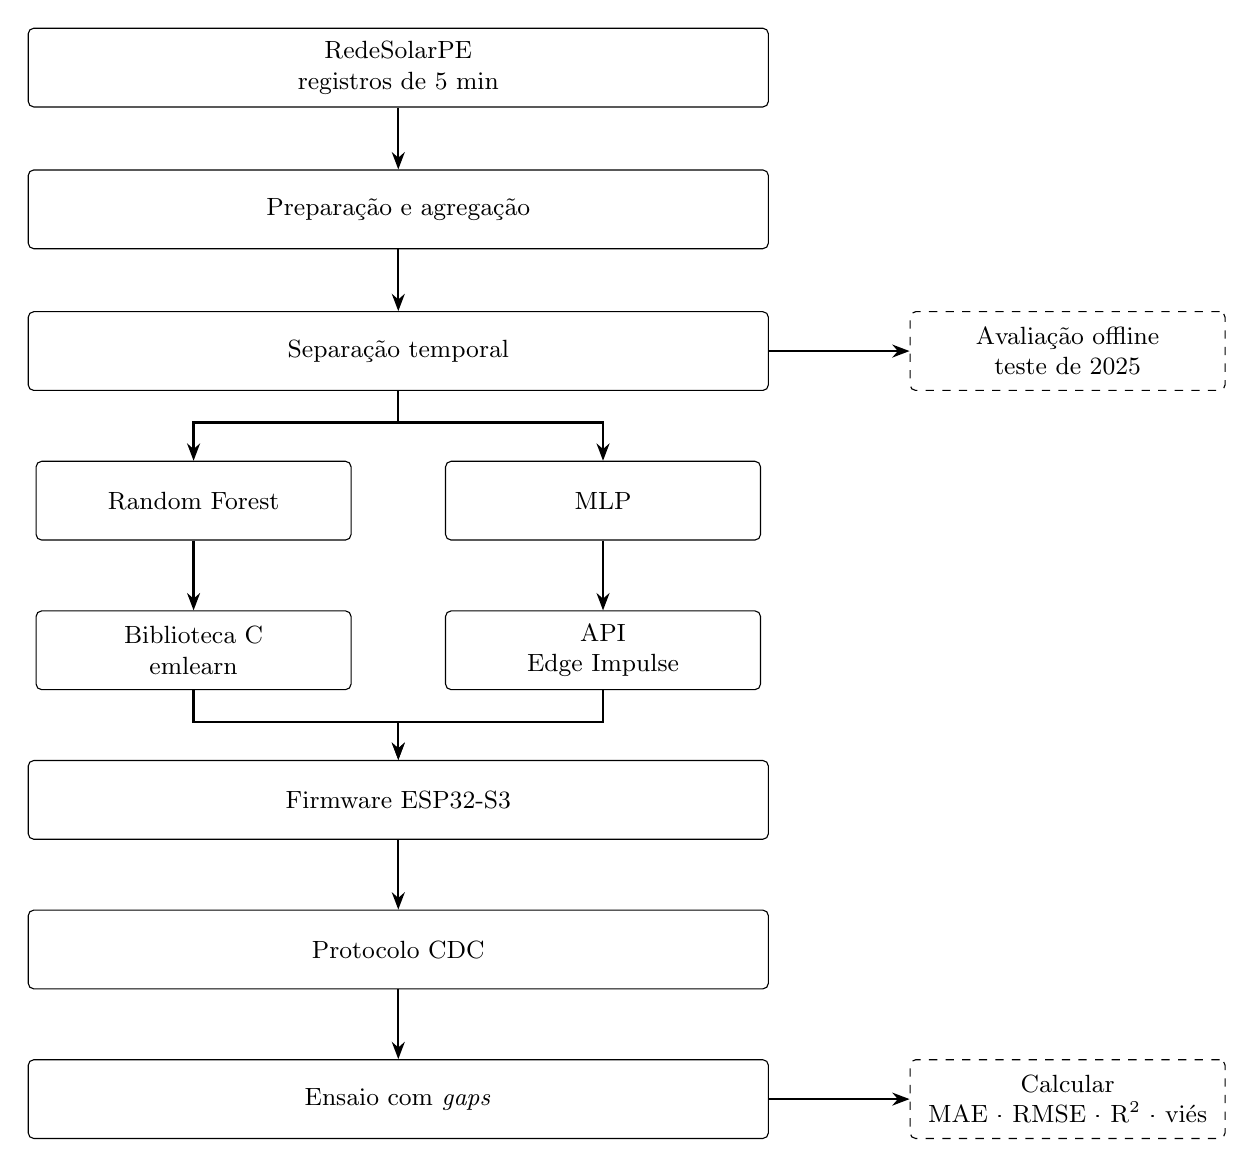
\begin{tikzpicture}[
      caixa/.style  = {draw, rectangle, rounded corners = 2pt, align = center,
                       minimum height = 10mm, minimum width = 40mm, font = \small},
      caixa larga/.style = {caixa, minimum width = 94mm},
      avaliacao/.style = {caixa, dashed},
      seta/.style   = {-{Stealth[length=2.2mm]}, thick}
    ]
    \node[caixa larga] (dados) at (0, 0) {RedeSolarPE\\registros de 5~min};
    \node[caixa larga] (prep) at (0, -1.8) {Preparação e agregação};
    \node[caixa larga] (split) at (0, -3.6) {Separação temporal};
    \node[avaliacao] (aval) at (8.5, -3.6) {Avaliação offline\\teste de 2025};
    \node[caixa] (rf) at (-2.6, -5.5) {Random Forest};
    \node[caixa] (mlp) at (2.6, -5.5) {MLP};
    \node[caixa] (lib) at (-2.6, -7.4) {Biblioteca C\\emlearn};
    \node[caixa] (ei) at (2.6, -7.4) {API\\Edge Impulse};
    \node[caixa larga] (firmware) at (0, -9.3) {Firmware ESP32-S3};
    \node[caixa larga] (protocolo) at (0, -11.2) {Protocolo CDC};
    \node[caixa larga] (ensaio) at (0, -13.1) {Ensaio com \textit{gaps}};
    \node[avaliacao] (coleta_res) at (8.5, -13.1) {Calcular \\MAE · RMSE · R$^2$ · viés};
    \draw[seta] (dados) -- (prep);
    \draw[seta] (prep) -- (split);
    \draw[seta] (split.south) -- ++(0,-0.4) -| (rf.north);
    \draw[seta] (split.south) -- ++(0,-0.4) -| (mlp.north);
    \draw[seta] (split.east) -- (aval.west);
    \draw[seta] (rf) -- (lib);
    \draw[seta] (mlp) -- (ei);
    \draw[seta] (lib.south) -- ++(0,-0.4) -| (firmware.north);
    \draw[seta] (ei.south) -- ++(0,-0.4) -| (firmware.north);
    \draw[seta] (firmware) -- (protocolo);
    \draw[seta] (protocolo) -- (ensaio);
    \draw[seta] (ensaio.east) -- (coleta_res.west);
  \end{tikzpicture}
  \source{Elaborado pelo autor.}
\end{figure}

\section{Conjunto de Dados}

\subsection{Base de Dados}

Os dados provieram da Rede Solarimétrica de Pernambuco (RedeSolarPE), rede
mantida pelo Instituto Federal de Pernambuco (IFPE), \textit{campus}
Pesqueira, que consolida em banco de dados centralizado registros operacionais
de usinas fotovoltaicas conectadas à rede no estado
\cite{pedrosafilho2022,pedrosafilho2025}. Desse conjunto, o estudo recortou a
planta do \textit{campus} Pesqueira, de 86~kWp, composta por 296 módulos de
245~Wp e 102 de 140~Wp \cite{moraesneto2024}, e utilizou três inversores de
2~kW denominados E1, E2 e E3, todos do mesmo modelo e fabricante, o que
reduziu diferenças de equipamento na comparação.  

A base de dados foi adquirida no formato de csv, totalizando 9 arquivos, 
cada arquivo contendo o histórico de um ano de cada inversor.
O inversor E1 é o único com histórico longo (2021--2025); E2 e E3 cobrem
2024--2025. Por ter a série mais extensa, E1 foi o inversor usado no treino, e
as cópias do último ano dos três permitiram avaliar a generalização entre
usinas. Os demais inversores da rede permaneceram fora do escopo deste
estudo.

As séries possuem resolução nativa de 5 minutos, contendo apenas registros
diurnos, filtrados pelo ângulo zenital solar $\leq 80^{\circ}$ na origem. O
alvo da regressão é a potência ativa CA (PCA, em kW) reportada pelo inversor. As
variáveis explicativas incluem a GHI transposta (\texttt{ghit}, em W/m$^2$),
a temperatura ambiente (\texttt{tem\_amb}) e a
temperatura do módulo estimada pelo modelo de Jacques (\texttt{jacques}),
além de índices de claridade (\texttt{kt}, \texttt{kc}) e temperaturas de
célula por modelos empíricos alternativos (\texttt{pvsyst\_cell},
\texttt{sandia}, \texttt{sandia\_cell}), disponíveis para a análise
exploratória.

O pipeline tratou $\text{PCA} = 0$ como sentinela de falha de telemetria,
não como medição de potência nula, e removeu os registros em saturação
($\text{PCA} \geq 2$~kW). Os zeros foram tratados no filtro de apagão e
excluídos do cálculo de erro.

\subsection{Análise Exploratória}

A análise exploratória precedeu a preparação dos dados e incluiu a inspeção das
séries históricas, a avaliação da integridade dos dados e da produtividade ao
longo do tempo. Também foram analisados o perfil horário e a autocorrelação da
potência, além do exame de sua distribuição em diferentes granularidades.

O perfil horário da potência por inversor confirmou o formato de sino esperado
da geração diurna, com valores baixos no início e no fim do dia e máximos
próximos ao meio-dia. A eficiência mensal $\text{PCA}/\text{ghit}$, razão que
elimina a sazonalidade do recurso solar, serviu como indicador de degradação do
sistema ao longo dos meses. Essa análise foi diagnóstica e não participou do
pipeline de treino.

A análise de integridade demonstrou que as séries apresentam lacunas: E1 tem
13{,}68\% dos períodos diurnos esperados sem registro; E2, 13{,}45\%; e E3,
13{,}43\%. A maior lacuna contínua observada foi de 12~h, e a pior cobertura
anual foi a do inversor E1 em 2022 (17{,}1\%). A implicação era que o modelo
precisava ser avaliado também nos períodos em que a telemetria faltava, o que
motivou o ensaio com \textit{gaps} artificiais descrito adiante. Além das
lacunas, 9\,607 leituras do conjunto bruto (2{,}3\%) registraram PCA igual a
zero.

Nesta etapa, também foi aplicada a função de autocorrelação parcial (PACF) e
a autocorrelação inversa (IACF) da série horária de PCA, além da análise da
distribuição do alvo e da matriz de correlação das variáveis meteorológicas. A
distribuição foi examinada em seis granularidades: 5~min, 10~min, 30~min, 1~h,
6~h e 1~d. Considerando que as leituras são apenas diurnas, 1~d corresponde a
cerca de 12~h de registro. A inspeção sustentou a decisão de não usar
variáveis defasadas e a escolha das features; a assimetria do alvo,
concentrado em valores baixos e com cauda até a saturação de 2~kW, motivou a
transformação de Box-Cox no caminho do MLP.

\subsection{Preparação dos Dados}

A preparação seguiu quatro etapas, aplicadas de forma idêntica às quatro
granularidades do desenho experimental (5~min, 10~min, 1~h e 1~d), de modo
que a comparação entre elas isolasse o efeito da agregação e não diferenças no
tratamento dos dados.

Etapa 1: carga e descarte. Os nove arquivos csv, com 410\,451 registros no
total, foram concatenados em um único conjunto; as colunas que não
participavam da modelagem foram descartadas e as 76 linhas sem valor de PCA
(NaN) foram removidas. As leituras com PCA igual a zero não foram descartadas
nesta etapa.

Etapa 2: filtros de qualidade. Antes da agregação, quatro tipos de registro
foram eliminados. O primeiro foi o apagão, definido como $\text{PCA} = 0$ com
$\text{ghit} > 50$~W/m$^2$: nesse caso, o inversor estava interrompido e a
relação irradiância--potência que se desejava modelar não se aplicava
\cite{severiano2026}. O segundo foi a baixa irradiância ($\text{ghit} < 5$~W/m$^2$),
que correspondia à noite ou ao início do dia, quando a potência era
praticamente nula e a medição não acrescentava informação. O terceiro foi a
temperatura ambiente acima de $50^{\circ}$C, atribuída a falha do sensor. O
quarto foi o filtro de saturação ($\text{PCA} \geq 2$~kW): os registros
foram removidos para que o patamar de recorte do inversor não fosse confundido
com a relação irradiância--potência que se desejava modelar
\cite{balfour2021}.

Etapa 3: agregação temporal. Os registros de 5~min foram agregados pela média
na granularidade desejada, pois o alvo era a potência média do período. As
leituras com PCA zero que restaram após o filtro de apagão, com irradiância de
até 50~W/m$^2$, foram mantidas: o critério de apagão só marcava o zero
acompanhado de irradiância alta. O Random Forest tratou esses valores
diretamente; no modelo de rede neural, um deslocamento de $0{,}001$~kW foi
somado ao alvo antes da transformação de Box-Cox \cite{boxcox1964}, que exigia
alvo estritamente positivo, e a inversa subtraiu o mesmo valor.

Etapa 4: separação temporal. O \textit{split} foi temporal e sem
embaralhamento: treino de 2021 até 30/06/2024, calibração no segundo semestre
de 2024 e teste em 2025, sempre com dados do E1. A divisão reservou o ano mais
recente para o teste e usou o semestre imediatamente anterior como janela de
calibração, em que o viés foi medido para posterior correção na implantação.
Cópias do ano de teste de cada inversor permitiram avaliar os modelos nos três
inversores no mesmo ano.

O contrato de modelagem foi fixado em um único módulo: três features
(\texttt{temperatura\_ambiente}, \texttt{ghit} e \texttt{jacques}, nessa
ordem), alvo \texttt{PCA}, índice temporal e semente aleatória 42. A ordem das
características fazia parte do contrato: trocá-la não provocava erro, apenas
predição errada e silenciosa, porque cada posição do vetor de entrada era
associada a uma grandeza diferente. Não havia colunas defasadas nem janelas de
entradas passadas: o alvo era a potência do mesmo período das entradas. A
fixação do contrato em um único módulo evitou que treino, avaliação e firmware
divergissem na ordem ou no conjunto de variáveis, um erro difícil de detectar
depois que o modelo já estava compilado.

\section{Treinamento dos Modelos}

Dois modelos, o Random Forest (RF) e o perceptron de múltiplas camadas (MLP),
foram treinados sobre o mesmo conjunto de dados, sob o mesmo
\textit{split} e com a mesma metodologia de avaliação, para permitir
comparação direta \cite{grinsztajn2022}. Todos os processos estocásticos
utilizaram a semente 42. Como linha de base, empregou-se uma regressão linear
múltipla com as mesmas características. A seleção de configurações foi
realizada exclusivamente na janela de calibração, nunca no conjunto de teste.
Os dois treinamentos percorreram as quatro granularidades do \textit{split} em
uma única execução; a biblioteca C embarcada no firmware foi gerada em etapa
separada, para a granularidade escolhida no ensaio.

\subsection{Random Forest}

O Random Forest \cite{breiman2001} foi treinado em cada granularidade. O
procedimento começou por uma varredura de 14 configurações de tamanho, de 300
árvores com mínimo de 2 amostras por
folha até 6 árvores com mínimo de 800, uma delas com teto de profundidade. A
varredura cobriu uma faixa ampla porque o tamanho adequado dependia da
granularidade: séries mais finas tinham mais amostras e suportavam árvores mais
profundas, enquanto séries grossas tinham poucas amostras e exigiam folhas
maiores para não memorizar o treino. Cada candidato foi avaliado pelo R$^2$ da
calibração já com o \textit{offset} do próprio candidato aplicado, uma vez
que o modelo entregue era sempre o calibrado; essa avaliação nunca usou o teste,
para não transformar a métrica final em treino disfarçado, e as colunas de
teste da varredura foram apenas reportadas.

Entre as duas configurações de maior R$^2$ calibrado, a seleção desempatou
pelo menor tempo de inferência por amostra, medido na validação, critério que
aproximava a escolha do custo real de operação. O desempate foi aplicado entre as
duas primeiras colocadas: como elas já estavam próximas em acurácia, preferiu-se
a mais rápida, que tendia a ter menos nós e a ocupar menos flash.
Em seguida, a floresta final foi treinada e salva em disco, para a análise
cruzada e para a geração posterior da biblioteca C, feita pelo script
\url{utils/gerar_lib_rf.py} com o \citeonline{emlearn2024}. O emlearn emitiu
o modelo como código \textit{inline}, e não como tabela em RAM, o que fez a
floresta não ocupar memória de dados. A configuração selecionada dependia da
granularidade: 10 árvores com mínimo de 300 amostras por folha em 5~min, 15
árvores com mínimo de 150 em 10~min, e 50 árvores com mínimo de 5 e teto de
profundidade 8 em 1~h e em 1~d.

A biblioteca gerada (\url{lib/knob-senses-rf/}) encapsulou o
pré-processamento: recebeu as três grandezas brutas, aplicou a normalização
\textit{z-score} com constantes gravadas na geração
(\url{normalizacao.json}) e devolveu a potência já limitada à faixa física
$[0, 2]$~kW. O viés residual foi corrigido pelo \textit{offset} medido na janela
de calibração. A normalização \textit{z-score} é dada por

\begin{equation}
\label{eq:zscore}
z = \frac{x - \mu}{\sigma},
\end{equation}
com $\mu$ e $\sigma$ calculados apenas sobre o treino. A biblioteca repetiu a
mesma operação antes de percorrer as árvores, e as constantes permaneceram
gravadas no arquivo de normalização e foram compiladas junto com o código;
assim, o firmware não lia JSON nem dependia de configuração externa.

A verificação foi dupla. Primeiro, o arquivo C gerado foi compilado no computador
de desenvolvimento e comparado ao modelo de origem do scikit-learn
\cite{pedregosa2011}; a comparação usou o mesmo conjunto de entrada e mediu a
diferença entre as predições das duas implementações. Em seguida, o código foi
compilado com a \textit{toolchain} xtensa para medir os custos reais de flash
e RAM do objeto gerado. A primeira verificação detectou erros de geração ou de 
normalização; a segunda, o custo real que o firmware pagaria.

\subsection{MLP}

O MLP foi implementado e treinado como uma rede densa do tipo
\textit{feedforward} no framework Keras \cite{chollet2015}. A arquitetura foi
composta por três camadas ocultas, com 128, 64 e 32 neurônios, respectivamente,
totalizando aproximadamente 10,9 mil parâmetros treináveis. Foram utilizadas
a função de ativação ReLU, uma taxa de \textit{dropout} de 0,1 e uma camada de
saída linear, cujo viés foi inicializado com a média do alvo transformado. A
ReLU foi escolhida por sua compatibilidade com a quantização em \textit{int8}.
A GELU, por sua vez, foi descartada nos testes, pois as operações envolvendo
a função de erro necessárias à sua implementação não possuem equivalente
inteiro no conversor do Edge Impulse.

As entradas foram normalizadas pelo método \textit{min-max}, cujos parâmetros
foram estimados exclusivamente com os dados de treino:

\begin{equation}
\label{eq:minmax}
x' = \frac{x - x_{\min}}{x_{\max} - x_{\min}}.
\end{equation}

A faixa resultante, $[0, 1]$, foi adotada para adequação à quantização em
\textit{int8}. Os valores mínimo e máximo foram determinados apenas a partir
do conjunto de treino e mantidos constantes durante a validação e o teste,
evitando o vazamento de informações entre os conjuntos.

Para viabilizar a transformação Box-Cox \cite{boxcox1964} das leituras nulas
de PCA preservadas no particionamento dos dados (\textit{split}), somou-se ao
alvo um deslocamento de $0{,}001$ kW. Em seguida, aplicou-se a transformação:

\begin{equation}
\label{eq:boxcox}
y^{(\lambda)} = \frac{y^{\lambda} - 1}{\lambda},
\end{equation}

em que $\lambda$ foi estimado exclusivamente com os dados de treino e
ajustado individualmente para cada granularidade. Antes da aplicação da
transformação inversa, as predições eram limitadas ao domínio válido da
inversa, definido pela condição $1 + \lambda y > 0$, considerando-se os
limites determinados a partir dos dados de treino.

A função de perda adotada foi a de Huber \cite{huber1964}, com limiar
$\delta$ definido como 0,25 vezes o intervalo interquartil (IQR) do alvo
transformado. O otimizador utilizado foi o Adam \cite{kingma2015}.

O treinamento foi validado na janela de calibração (2024H2), que também foi
utilizada para estimar o viés, e realizado sem embaralhamento das amostras.
Dois \textit{callbacks} foram empregados para controlar a convergência. O
primeiro, de parada antecipada (\textit{early stopping}), monitorou o erro
absoluto médio (MAE) na validação e restaurou os pesos correspondentes à
melhor época \cite{prechelt1998}. Sua paciência foi definida como o dobro do
valor indicado na coluna correspondente da
\cref{tab:hiperparametros}. O segundo, de redução da taxa de aprendizado por
platô (\textit{reduce learning rate on plateau}), reduziu essa taxa pela
metade quando não houve melhora no MAE de validação durante oito épocas
consecutivas, respeitando o limite mínimo de $10^{-8}$.

Os demais hiperparâmetros foram definidos de acordo com a granularidade,
conforme apresentado na \cref{tab:hiperparametros}. Em geral, as granularidades
mais finas utilizaram lotes maiores e taxas de aprendizado menores, enquanto
as mais grossas empregaram lotes menores, maior número de épocas e taxas de
aprendizado mais elevadas.

\begin{table}[H]
    \centering
    \caption{Hiperparâmetros do MLP por granularidade}
    \label{tab:hiperparametros}
    \begin{tabular}{lcccc}
        \toprule
        Granularidade & Épocas & \textit{Batch} & Paciência &
        Taxa de aprendizado \\
        \midrule
        5 min  & 400 & 512 & 60 & $3\times10^{-4}$ \\
        10 min & 400 & 256 & 60 & $3\times10^{-4}$ \\
        1 h    & 300 & 64  & 40 & $5\times10^{-4}$ \\
        1 d    & 600 & 32  & 60 & $1\times10^{-3}$ \\
        \bottomrule
    \end{tabular}
    \source{Elaborado pelo autor.}
\end{table}

O pós-processamento foi realizado por meio de uma sequência fixa de operações,
cujos parâmetros foram armazenados em
\url{dist/{freq}/transformacao_alvo.json}, com um arquivo para cada
granularidade. Primeiro, a predição no espaço transformado foi limitada ao
domínio válido da transformação e submetida à inversa de Box-Cox. Em seguida,
subtraiu-se o deslocamento de $0{,}001$ kW aplicado ao alvo na etapa de
preparação dos dados. Depois, adicionou-se o \textit{offset} de calibração
estimado na janela 2024H2. Por fim, o resultado foi limitado à faixa física
de $[0, 2]$ kW. Essa ordem foi necessária para garantir a validade matemática
da transformação inversa e a consistência das operações seguintes, uma vez
que tanto o deslocamento inicial quanto o \textit{offset} de calibração são
expressos na unidade física do alvo. A limitação final assegurou que nenhuma
predição ultrapassasse os limites físicos estabelecidos.

Para a execução embarcada, o modelo foi exportado no formato SavedModel e
convertido para TensorFlow Lite \cite{abadi2016}. O script
\url{utils/exportar_mlp_ei.py} automatizou o envio do modelo ao Edge Impulse
Studio \cite{edgeimpulse2024,tflitemicro2024} e o posterior download da
biblioteca C++ compilada pela plataforma, utilizando a amostra de calibração
e os parâmetros de normalização estimados no treino. Essa biblioteca reuniu
o SDK de inferência, os parâmetros do modelo e o código gerado pelo Studio,
sendo instalada diretamente em \url{lib/knob-senses/}.

\subsection{Avaliação e Métricas}

Os modelos foram avaliados no \textit{split} de teste de cada granularidade, com
as métricas usuais em estimação de potência fotovoltaica
\cite{chicco2021,hodson2022}. A avaliação usou o mesmo conjunto para os dois
modelos e para a regressão linear, para que as diferenças observadas
fossem atribuídas ao modelo e não ao tratamento dos dados: o erro absoluto
médio,

\begin{equation}
\label{eq:mae}
\mathrm{MAE} = \frac{1}{n} \sum_{i=1}^{n} \left| y_i - \hat{y}_i \right|,
\end{equation}
a raiz do erro quadrático médio,

\begin{equation}
\label{eq:rmse}
\mathrm{RMSE} = \sqrt{\frac{1}{n} \sum_{i=1}^{n} \left( y_i - \hat{y}_i \right)^{2}},
\end{equation}
o coeficiente de determinação,

\begin{equation}
\label{eq:r2}
R^{2} = 1 - \frac{\sum_{i=1}^{n} \left( y_i - \hat{y}_i \right)^{2}}
                {\sum_{i=1}^{n} \left( y_i - \bar{y} \right)^{2}},
\end{equation}
o erro percentual absoluto médio,

\begin{equation}
\label{eq:mape}
\mathrm{MAPE} = \frac{100}{n} \sum_{i=1}^{n} \left| \frac{y_i - \hat{y}_i}{y_i} \right|,
\end{equation}
e o viés (erro sistemático),

\begin{equation}
\label{eq:vies}
\text{viés} = \frac{1}{n} \sum_{i=1}^{n} \left( \hat{y}_i - y_i \right),
\end{equation}
em que $y_i$ e $\hat{y}_i$ são a potência medida e a estimada da $i$-ésima
amostra, e $\bar{y}$ a média das medições. Complementaram a avaliação o
percentil 90 do erro absoluto (p90) e o teto (maior predição e quantas
amostras a atingem). Linhas com PCA zero (sentinela) ou sem valor (NaN)
ficaram fora do cálculo de erro, por serem rótulos inválidos.

Além da avaliação na própria granularidade, uma análise cruzada aplicou cada
modelo treinado ao teste das demais granularidades, formando uma matriz em
que a linha era a granularidade de treino e a coluna, a de avaliação. O
objetivo era verificar se o modelo dependia da resolução em que foi treinado ou
se podia ser aplicado a outra. As
entradas do teste foram reescaladas com as constantes de normalização do
treino, fora da faixa $[0, 1]$ quando a granularidade de avaliação era mais
fina que a de treino, o que mediu justamente a capacidade de extrapolação do
modelo. A diagonal da matriz correspondia ao próprio modelo; abaixo dela estava
o cenário de interesse, o modelo grosso avaliado em dado fino.

\section{Implantação Embarcada}

O alvo de implantação foi o ESP32-S3 \cite{espressif2024}. O projeto usou o
PlatformIO com um ambiente por modelo \cite{platformio2024}: os
\textit{envs} \texttt{rf} e \texttt{mlp} definiram a macro
\texttt{-DMODEL\_*} que seleciona em tempo de compilação a biblioteca
embarcada correspondente, e cada firmware continha apenas o modelo e as
dependências do seu caminho; upload e monitoração eram comuns aos dois.
Cada modelo foi compilado em firmware próprio e ensaiado isoladamente,
seguindo o procedimento de \citeonline{moraesneto2024}.

A geração do artefato foi acoplada ao build, mas só executava quando necessária.
O gancho de pré-compilação (\url{scripts/pre_build.py}), ligado aos dois
ambientes por \texttt{extra\_scripts}, rodava na carga do script do
PlatformIO, antes de o grafo de compilação ser montado, e não como uma ação
do SCons, que só dispararia quando houvesse algo a recompilar. Ele guardava em
\url{.pio/prebuild/{env}.json} a assinatura do artefato usado na última
geração (data de modificação e tamanho) e a granularidade embarcada.

Antes de compilar, comparava a assinatura com a do arquivo do modelo em disco: se nada
mudou, mantinha a biblioteca existente e seguia o build; se o modelo ou a
granularidade mudaram, executava \url{utils/gerar_lib_rf.py} ou
\url{utils/exportar_mlp_ei.py} para a granularidade configurada nas opções do
projeto (\texttt{custom\_rf\_freq} e \texttt{custom\_mlp\_freq}, com valores
válidos 5min, 10min, 1h e 1D). Uma falha no script interrompia o build, para não
embarcar uma biblioteca desatualizada; a variável de ambiente
\texttt{KNOB\_SKIP\_PREBUILD} dispensava a etapa, por exemplo para compilar sem
rede até o Edge Impulse.

O firmware era um cliente de teste que não lia sensores: recebia lotes de amostras
do servidor, executava a inferência de cada uma e devolvia as predições em lote
pela CDC do controlador USB-Serial do próprio ESP32-S3, com o log de
execução mantido na UART0. O gancho de inferência (\texttt{runInference()}) era
o ponto de aquisição (em campo, era ali que entravam os sensores da usina, sem
alterar o restante do pipeline). As constantes
de operação (1 amostra, 3 eixos, quadro de 3 \textit{floats}) vinham dos
cabeçalhos gerados de cada modelo; o período nominal de inferência (10~ms no
RF e 1~ms no MLP) era o ritmo da operação em tempo real, e o ensaio o dispensava,
andando na velocidade dos lotes.

O contrato de normalização era explícito: o firmware sempre entregava grandezas
brutas. No caminho RF, a normalização acontecia dentro da biblioteca; no
caminho MLP, o SDK do Edge Impulse aplicava o escalonador embutido no impulso.
A arena de memória do TensorFlow Lite era de 3\,174~bytes; o RF era código
\textit{inline}, sem tabela em RAM, com custo de flash medido no objeto
compilado. O laço de execução registrava atrasos de período
(\textit{overruns}) e falhas de troca (\textit{dropouts}, com retentativa
da mesma amostra), tratava erro de inferência como fatal e monitorava o heap
livre a cada predição, para detectar fragmentação de memória.

\section{Protocolo de Comunicação}

O ensaio na placa usou mensagens binárias \textit{little-endian}
(\cref{tab:protocolo}) sobre a CDC do controlador USB-Serial do
ESP32-S3, organizadas em lotes. Em vez de duas transferências por linha, o
servidor enviava um lote de até 64 amostras numa escrita só e recebia as
predições correspondentes numa leitura só. O lote respondia a uma medição
de bancada: o enlace apresentava pausas de cerca de 2~s a cada dezenas de
mensagens pequenas, e o lote amortizava cada pausa por até 64 linhas, o que
reduzia o tempo total do ensaio. Um \textit{handshake} de um byte de
sincronização marcou o início de cada sessão e deixou para trás os resíduos do
\textit{bootloader} escritos na porta antes do ensaio, em duas variantes:
\texttt{0x52} (\texttt{RESET}), usado uma vez por usina, e \texttt{0x4B}
(\texttt{RESUME}), usado nas retomadas, pois o host reenviava o byte até a
resposta chegar; o firmware descartava os bytes que sobrassem na fila atrás
dele. O lote endereçava as linhas do teste pela base, que era a primeira linha,
e pelo tamanho \texttt{n}, e o firmware era apátrida por lote: quem controlava o
andamento do ensaio era o servidor, e um lote reenviado reprocessava exatamente
as mesmas amostras.

\begin{table}[H]
  \centering
  \caption{Mensagens do protocolo de ensaio}
  \label{tab:protocolo}
  \begin{tabular}{llrp{6.2cm}}
    \toprule
    Mensagem & Sentido & Bytes & Descrição \\
    \midrule
    Lote de amostras & servidor $\rightarrow$ ESP32 & $9 + 12n$ & \texttt{0x01} + base (u32) + $n$ (u32) + $n \times 3$ \texttt{float32} \\
    Lote de predições & ESP32 $\rightarrow$ servidor & $9 + 4n$ & \texttt{0x03} + base (u32) + $n$ (u32) + $n \times$ \texttt{float32} \\
    Fim do dataset & servidor $\rightarrow$ ESP32 & 9 & \texttt{0x01} + base + $n = 0$ \\
    \bottomrule
  \end{tabular}
  \source{Elaborado pelo autor.}
\end{table}

O servidor tolerava reconexão: o estado do ensaio era o lote pendente, não o
meio. O \textit{timeout} de leitura era assimétrico, 2~s no firmware e 5~s no
servidor, para que o cliente sempre desistisse primeiro e não ficasse esperando
uma resposta que o servidor já abandonou. Quando a leitura do servidor
estourava, o \textit{handshake} \texttt{RESUME} refazia a sessão e o servidor
reenviava o mesmo lote, idempotente por construção. O ensaio terminava com um
lote vazio ($n$~=~0), após o qual o firmware se re-armava e aguardava o
\texttt{RESET} da próxima usina.

\section{Ensaio na Placa}

O servidor de teste (\url{notebooks/model_teste.ipynb}) abriu a porta CDC do
USB\-Serial e serviu as linhas do \textit{split} de teste da granularidade
do ensaio, endereçadas pela base do lote, na ordem das características do
contrato. Cada predição confirmada virava uma linha
\url{sample, real, pred, err} no log do ensaio, que servia tanto para o
acompanhamento durante a execução quanto para a análise posterior. A
exclusividade do meio era natural: a porta serial não admitia duas aberturas.
Um ensaio foi executado por inversor, usando as cópias do ano de teste de cada
usina, o que permitiu comparar os três no mesmo período.

O ensaio avaliou o soft-sensor no cenário de falha de telemetria do inversor.
O servidor introduziu \textit{gaps} artificiais nos três inversores antes de
servir os dados: blocos contíguos de 1~h, 6~h, 24~h e 3 dias, com quatro
blocos de cada duração que coubesse na granularidade do ensaio, e uma fração
aleatória de 10\% das leituras restantes. A fração ocultada ficou entre 16\%
e 20\% das leituras.

Nas linhas de \textit{gap} apenas o PCA foi ocultado, pois
as variáveis meteorológicas vinham de outro sistema de medição e seguiam
disponíveis, e o valor verdadeiro permanecia guardado para a validação. O
firmware não mudou: recebia as características, inferia e devolvia a predição.

A validação mediu o erro em dois conjuntos. Fora dos \textit{gaps}, a
comparação foi a usual entre o estimado e o medido. Dentro deles, a comparação
foi entre a estimativa do soft-sensor e o valor real oculto, com as métricas
desagregadas por duração do bloco. A estimativa foi comparada com a
interpolação linear, que usa os dois lados do buraco, e com a persistência do
último valor observado. O soft-sensor foi considerado viável se o seu erro
dentro dos \textit{gaps} fosse igual ou menor que o da interpolação linear e
permanecesse próximo do erro fora deles.

A matriz experimental (\cref{tab:matriz}) definiu oito ensaios E1--E8,
cobrindo os dois modelos nas quatro granularidades, repetidos nos três
inversores. O desenho permitiu comparar o custo embarcado e a acurácia de cada
combinação no mesmo cenário de falha, e não apenas no teste
\textit{offline}. O procedimento de cada ensaio foi: (i) gerar o artefato do
modelo na granularidade, a biblioteca C do RF ou o impulso do Edge Impulse,
reexportado no Studio com os dados e o contrato daquela granularidade; (ii)
gravar o firmware do \textit{env} correspondente; (iii) subir o servidor de
teste, que gerava os \textit{gaps}; e (iv) reiniciar a placa e deixar o ensaio
rodar até o fim do dataset, com as métricas calculadas ao final. Antes de
transmitir, a ordem dos eixos era conferida entre o servidor e a normalização
da biblioteca (\texttt{check\_axis\_order()}), pois a troca de ordem produzia
predição errada sem erro. Uma limitação conhecida: reiniciar o servidor no
meio do ensaio zerava o log; para recomeçar do zero, subia-se o servidor e
reiniciava-se a placa.

\begin{table}[H]
  \centering
  \caption{Matriz experimental dos ensaios na placa}
  \label{tab:matriz}
  \begin{tabular}{lcccc}
    \toprule
    Modelo & 5 min & 10 min & 1 h & 1 d \\
    \midrule
    Random Forest & E1 & E2 & E3 & E4 \\
    MLP & E5 & E6 & E7 & E8 \\
    \bottomrule
  \end{tabular}
  \source{Elaborado pelo autor.}
\end{table}

\chapter{Resultados}
\label{cap:resultados}

Texto.

% ============================================================================
% RASCUNHO COMENTADO: Conclusão
% Para publicar, remova o "%" do início de cada linha.
% ============================================================================
\chapter{Conclusão}
\label{cap:conclusao}

% O trabalho partiu de um problema prático: quando a telemetria de um
% inversor fotovoltaico falha, a potência gerada deixa de ser registrada, e
% a lacuna compromete o acompanhamento da usina. A proposta foi reconstruir
% essa potência a partir de variáveis meteorológicas medidas de forma
% independente, com um soft-sensor embarcado, e avaliar o resultado tanto no
% computador quanto no hardware que seria usado em campo.
%
% O pipeline cobriu a preparação dos dados em quatro granularidades, o
% treino do Random Forest e do MLP, a geração das bibliotecas embarcadas, o
% firmware e o ensaio na placa. A comparação controlada mostrou que o MLP
% tem o menor erro em todas as granularidades e que o Random Forest fica
% próximo, com diferença pequena em favor da rede neural. O Random Forest
% leva vantagem no custo embarcado, por ser código \textit{inline} sem arena
% de memória. A regressão linear de referência fica bem abaixo, sobretudo em
% 1~d, com R$^2 = 0{,}534$.
%
% A análise cruzada de granularidades mostrou que a resolução de treino não
% prende o modelo à resolução de operação. Um modelo treinado em 1~h e
% avaliado em 5~min mantém R$^2$ de $0{,}784$ (MLP) e $0{,}777$ (RF); o
% modelo treinado em 1~d perde mais ao descer para o dado fino, com
% $0{,}696$ e $0{,}640$, mas se recupera em 1~h. Isso dá flexibilidade ao
% projeto, ao custo de uma perda que cresce com a distância entre as
% granularidades.
%
% O ensaio E3, com o Random Forest de 1~h na ESP32-S3, percorreu as 4\,042
% linhas do teste de 2025 do inversor E1. Fora dos \textit{gaps}, o caminho
% embarcado reproduziu o modelo treinado, com MAE de $0{,}066$~kW, RMSE de
% $0{,}083$~kW, R$^2$ de $0{,}972$ e viés de $+0{,}003$~kW. Dentro dos
% \textit{gaps}, o MAE foi de $0{,}065$~kW, enquanto a interpolação linear
% errou $0{,}312$~kW e a persistência, $0{,}376$~kW. Os números mostram a
% viabilidade do soft-sensor como complemento ao medidor: o erro dentro dos
% \textit{gaps} fica próximo do erro normal e muito abaixo das alternativas
% clássicas, que pioram à medida que o buraco cresce.
%
% As contribuições do trabalho são o pipeline completo, do dado bruto ao
% ensaio embarcado; a comparação controlada entre um modelo de árvores e uma
% rede neural nas mesmas condições; a análise cruzada de granularidades; o
% ensaio com \textit{gaps} artificiais e baselines de imputação; e a
% automação da geração dos artefatos no build.
%
% O trabalho tem limitações claras. Apenas o ensaio E3 foi executado; os
% ensaios E1, E2 e E4 a E8 e os inversores E2 e E3 permanecem pendentes. O
% ensaio é \textit{offline}: o firmware recebe lotes do servidor em vez de
% ler sensores. Os \textit{gaps} são artificiais, não falhas reais de
% telemetria. A calibração usa apenas o segundo semestre de 2024, e o
% estudo cobre um \textit{campus} e inversores de 2~kW. Essas limitações
% delimitam o alcance dos resultados, mas não mudam o que foi observado no
% ensaio executado.
%
% Os desdobramentos naturais são completar a matriz experimental e ensaiar
% os três inversores; levar o firmware para campo, com os sensores reais;
% comparar outras arquiteturas e outras formas de quantização; e integrar o
% soft-sensor ao sistema de aquisição da usina, para que a estimativa seja
% produzida no momento da falha e registrada junto com a série medida.


% ----------------------------------------------------------
% ELEMENTOS PÓS-TEXTUAIS
% ----------------------------------------------------------
\postextual
\bibliography{referencias}

\end{document}
